\chapter{De naturlige tal}

Alle kender de naturlige tal, selv om man måske ikke ved, at de hedder netop dét. De naturlige tal er tallene
%
\[ 1, 2, 3, 4, 5, 6, 7, 8, 9, 10, 11 \ldots \]
%
Hvorfor kaldes de naturlige tal \emph{naturlige}? Begrebet er i al fald gammelt. Ordet dukker op i 1763 i \emph{The method of increments} af den engelske matematiker William Emerson, der taler om 
\begin{quote}
    To find the product of all natural numbers from 1 to 100 \ldots
\end{quote}
men der er også tidligere anvendelser, hvor matematikerne siger, at der er noget særligt "naturligt" ved netop denne slags tal.

Hvad er det, der er så naturligt her? Måske fordi der er tale om den fiktion om tal, der naturligt falder mennesker ind. Børn lærer at tælle, længe før de lærer om de negative tal, for slet ikke at tale om brøkerne.

Den store tyske matematiker Leopold Kronecker er kendt for at have sagt (i en korrespondance med sin kollega og landsmand Ferdinand Lindemann) at

\begin{quote}
    Die ganzen Zahlen hat der liebe Gott gemacht, alles andere ist Menschenwerk. 
\end{quote}

eller oversat til på dansk

\begin{quote}
    De hele tal har den kære Gud skabt, alt andet er menneskeværk.
\end{quote}

Kronecker mente således, at matematikken er menneskers værk -- en fiktion. Men hvem skabte de naturlige tal? Det var såmænd den italienske matematiker Giuseppe Peano.

\section{Peanos aksiomer}

\begin{figure}[h]
    \centering
    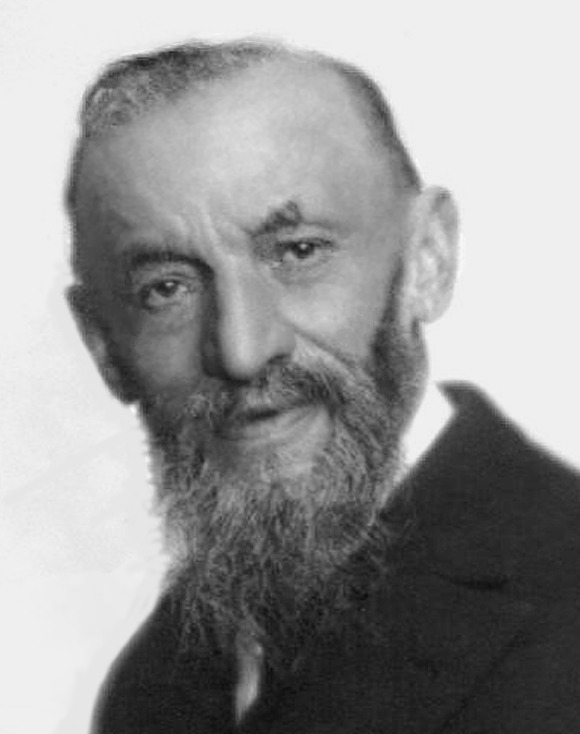
\includegraphics[width=6cm]{GiuseppePeano.jpg}
    \caption{Giuseppe Peano}
    \label{fig:peano}
\end{figure}

Den italienske matematiker Giuseppe Peano (1858-1932) gav en definition af de naturlige tal, der har vundet indpas i matematik, nemlig det, vi i dag kender som Peanos aksiomer. Peanos aksiomer fortæller os, at de naturlige tal er de tal, vi kan nå ved at starte ved $0$ og tælle opad. Og de lyder sådan:

\begin{enumerate}
    \item $0$ er et naturligt tal
    \item Hvis $n$ er et naturligt tal, er efterfølgeren $S(n)$ også et naturligt tal
    \item Der findes ikke andre naturlige tal end disse.
\end{enumerate}

Efterfølgerfunktionen $S$ skal man blot tænke på som et "flag" vi sætter foran. Ofte vil man skrive $n+1$ i stedet for $S(n)$, og det vil vi også af og til gøre i det følgende.

Tallet $2$ kan vi repræsentere som $S(S(0))$, dvs. ved at sætte $2$ $S$'er foran $0$. Og tallet $16$ kan vi på tilsvarende vis repræsentere som
%
\[ S(S(S(S(S(S(S(S(S(S(S(S(S(S(S(S(0))))))))))))))))\]
%
Læseren vil med lidt tålmodighed nemt kunne finde repræsentationen af $484719$.

\section{Addition}

Vi kender godt regningsarterne. Hvis vi vil definere addition, kan vi gøre det således.

\begin{enumerate}
    \item \label{plus-1} $0 + n = n$
    \item \label{plus-2} $S(n) + m = S(n+m)$
\end{enumerate}

Dette er endnu en fiktion om de naturlige tal.

\subsection{At vise at $2+2 = 4$}

Hvad er $2+2$? Husk at $2$ er $S(S(0))$. Så spørger vi, hvad $S(S(0)) + S(S(0))$ er. Her kan vi bruge vores fiktion om addition, undskyld vores definition af $+$.

Hvis vi sætter ind i betingelse \ref{plus-2}, får vi os at 
%
\[ S(S(0)) + S(S(0)) = S(S(0) + S(S(0)))  \]
%
og ved igen at sætte ind i betingelse \ref{plus-2}, får vi os at 
%
\[  S(S(0) + S(S(0))) = S(S(S(0 + S(0)))) \]
%
Så kan vi bruge betingelse \ref{plus-1}, og den giver os ved indsætning at
%
\[ S(S(S(0 + S(0)))) = S(S(S(S(0)))) \]
%
Så resultatet er $S(S(S(S(0))))$, dvs. tallet $4$. Med andre ord: Vi har nu vist at $2+2 = 4$.

\section{For alle naturlige tal gælder at \ldots}

Peano angav også en metode til at bevise, at en påstand gælder for alle naturlige tal. 

\begin{quote}
Lad $P$ være en påstand.
    \begin{enumerate}
    \item Hvis påstanden $P$ gælder for $0$
    \item Og hvis vi kan vise, at hvis påstand $P$ gælder for et naturligt tal $n$, da gælder $P$ også for $S(n)$    
\end{enumerate}
Da ved vi at påstanden $P$ gælder for alle naturlige tal
\end{quote}

Denne bevisteknik kalder man i dag for \emph{matematisk induktion}. Teknikken er meget ældre end Peano; den skyldes en anden italiener, Francesco Maurolico, der i sin bog \emph{Arithmeticorum libri duo} fra 1575 bruger matematisk induktion til at vise at summen af de første $n$ ulige tal:
%
\[ 1 + 3 + \cdots + (2n-1)  \]
%
er $n^2$. 

Matematisk induktion består i at vise at vores påstand gælder for det mindste naturlige tal, nemlig $0$ - det kalder vi for \emph{basistilfældet}. Og vi skal derefter vise, at påstanden bliver ved med at gælde, når vi giver os til at tælle -- det kalder vi for \emph{induktionsskridtet}.

Man kan også starte længere fremme i den naturlige talrække end ved $0$. Hvis man vil vise at en påstand $P$ gælder for alle naturlige tal der er større end eller lig $k$, skal vi bare vise at 

 \begin{enumerate}
    \item Påstanden $P$ gælder for $k$ (så $k$ er nu basistilfældet)
    \item Hvis påstanden $P$ gælder for et naturligt tal $n$, da gælder $P$ også for $S(n)$    
\end{enumerate}

Lad os se, hvad Maurolico gjorde, og lad os beskrive det, som Peano ville have gjort det.

Påstanden $P$ er altså at 
%
\[ 1 + 3 + \cdots + (2n+1) = n^2  \;\text{for}\; n \geq 1\]
%
Først skal vi vise basistilfældet, nemlig at summen af de første $1$ naturlige tal er $1^2$. Men det er oplagt, for $1 = 1^2$.

Så kommer skridtet. Vi skal vise, at hvis påstanden $P$ gælder for $n$, så gælder den også for $n+1$.

Påstanden $P$ gælder for $n$ præcis når
%
\[ 1 + 3 + \cdots + (2n-1) = n^2 \]
%
Det næste ulige naturlige tal efter er $(2n-1) + 2$. Så vi skal vise at
%
\[  1 + 3 + \cdots + (2n-1) + ((2n-1)+2) = (n+2)^2 \] 
%
Men betragt summen 
%
\[  1 + 3 + \cdots + (2n-1) + ((2n-1)+2)\] 
%
Den kan skrives som 
%
\[  (1 + 3 + \cdots + (2n-1)) + ((2n-1)+2) \] 
%
Hvis vi antager at påstanden $P$ gælder for $n$, har vi at
%
\[ 1 + 3 + \cdots + (2n-1) = n^2 \]
%
men så ved vi at
%
\[  (1 + 3 + \cdots + (2n-1)) +  ((2n-1)+2) = n^2 + ((2n-1)+2) \] 
%
Men 
\[ (n+1)^2 = n^2 + 2n + 1 \]
og
\[  n^2 + ((2n-1)+2) = n^2 +2n + 1 = (n+1)^2 \] 
hvilket afslutter beviset.

\section{Vores fiktion om addition ligner addition!}

En af de helt grundlæggende love, som skal gælde om addition, er at det er ligegyldigt i hvilken rækkefølge vi lægger tal sammen. Vi vil rigtig gerne have, at f.eks. $2+3 = 3+2$. Denne lov kalder man ofte for \emph{den kommutative lov}. 

Lad os prøve at vise at den kommutative lov gælder for de naturlige tal, dvs. at $m+n = n +m$ for alle naturlige tal $m$ og $n$.

Vi viser

\begin{paastand}
For ethvert naturligt tal $m$ gælder det, at det for ethvert naturligt tal $n$ gælder at $m + n = n + m$.
\end{paastand}

Dette er en påstand om alle naturlige tal $m$, så for at vise den, bruger vi matematisk induktion for $m$.

Først skal vi vise påstanden for $m = 0$, dvs. at $0+n=n+0$.

Men det er jo også en påstand om alle naturlige tal. Den hedder

\begin{paastand}\label{paa:to}
For alle naturlige tal $n$ gælder at $0+n=n+0$.
\end{paastand}

så den skal vises også. Så her skal vi også bruge matematisk induktion for at vise Påstand \ref{paa:to}.

Så lad os vise Påstand \ref{paa:to} først. Først skal vi vise, at $0+0=0+0$, men det gælder jo umiddelbart.

Så antager vi, at $0+n = n+0$ og skal med den antagelse i baglommen vise, at så gælder det også at $0 + (n+1) = (n+1) + 0$. Men $(n+1) + 0 = (n+0)+1$ ifølge vores definition af addition. Og da $n+0 = n$, må vi have at $(n+1) + 0 = n +1 $. Pr. definition af addition har vi at $0 + (n+1) = n+1$, og nu kan vi se, at påstanden gælder.

\section{\ldots men hvad med subtraktion?}

Når man har sagt plus, siger man også på et eller andet tidspunkt minus -- eller subtraktion, som det også kaldes.

Vi ved, at de naturlige tal ikke er \emph{lukket under} subtraktion. For $1-2$ er ikke et naturligt tal. Løsningen på det er enkel: Vi indfører de negative tal.

Så de negative tal er endnu en fiktion.